\documentclass[a4paper,11pt,twoside]{article}
%\documentclass[a4paper,11pt,twoside,se]{article}

\usepackage{UmUStudentReport}
\usepackage{verbatim}   % Multi-line comments using \begin{comment}
\usepackage{courier}    % Nicer fonts are used. (not necessary)
\usepackage{pslatex}    % Also nicer fonts. (not necessary)
\usepackage[pdftex]{graphicx}   % allows including pdf figures
\usepackage{listings}
\usepackage{pgf-umlcd}
%\usepackage{lmodern}   % Optional fonts. (not necessary)
%\usepackage{tabularx}
%\usepackage{microtype} % Provides some typographic improvements over default settings
%\usepackage{placeins}  % For aligning images with \FloatBarrier
%\usepackage{booktabs}  % For nice-looking tables
%\usepackage{titlesec}  % More granular control of sections.

% DOCUMENT INFO
% =============
\department{Department of Computing Science}
\coursename{C Programming and Unix 7.5 p}
\coursecode{5DV088}
\title{mfind}
\author{Lorenz Gerber ({\tt{dv15lgr@cs.umu.se}} {\tt{lozger03@student.umu.se}})}
\date{2016-10-17}
%\revisiondate{2016-01-18}
\instructor{Mikael Ränner / Filip Åberg / Jonathan Westin / Mattias Åsander}


% DOCUMENT SETTINGS
% =================
\bibliographystyle{plain}
%\bibliographystyle{ieee}
\pagestyle{fancy}
\raggedbottom
\setcounter{secnumdepth}{2}
\setcounter{tocdepth}{2}
%\graphicspath{{images/}}   %Path for images

\usepackage{float}
\floatstyle{ruled}
\newfloat{listing}{thp}{lop}
\floatname{listing}{Listing}



% DEFINES
% =======
%\newcommand{\mycommand}{<latex code>}

% DOCUMENT
% ========
\begin{document}
\lstset{language=C}
\maketitle
\thispagestyle{empty}
\newpage
\tableofcontents
\thispagestyle{empty}
\newpage

\clearpage
\pagenumbering{arabic}

\section{\textit{mfind} and Thread Safety} 

The scheme in figure 1 shows the most important aspects of the mfind system and how it was implemented here. It can be basically seen as a producer consumer system, however, each thread can be both producer and consumer. The most important source of synchronization is the semaphore which distributes the jobs to the threads. When there are no more jobs available. The `do while' loop looks futile on the first view, however, new jobs can be added after passing the `no wait' semaphore until checking the value of the semaphore in the `while' expression.

\begin{figure}
\centering
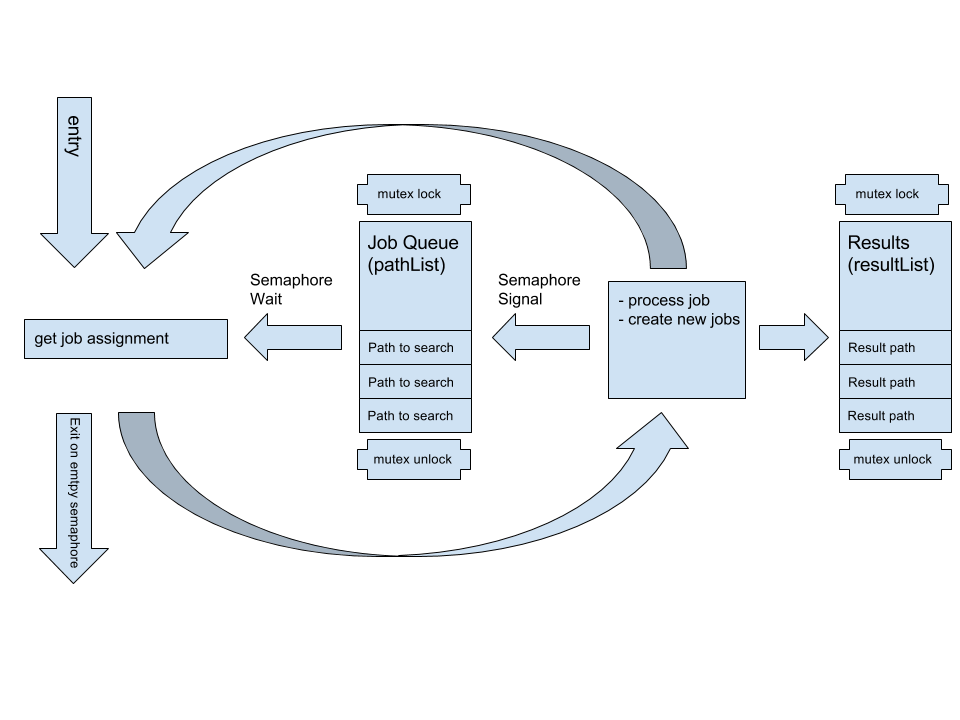
\includegraphics[width=\textwidth]{schema.png}
\caption{\textit{This figure shows a schematic view of the mfind problem.}}
\label{fig:scheme}
\end{figure}

The current construction is thread safe: The last thread in the loop can not leave until all jobs, also freshly self created are processed. In certain cases, this could lead to an uneven workload. This could be addressed by further synchronizing the threads, however this would also affect performance for most general cases. 


\section{Performance Assessment}

\begin{figure}
\centering
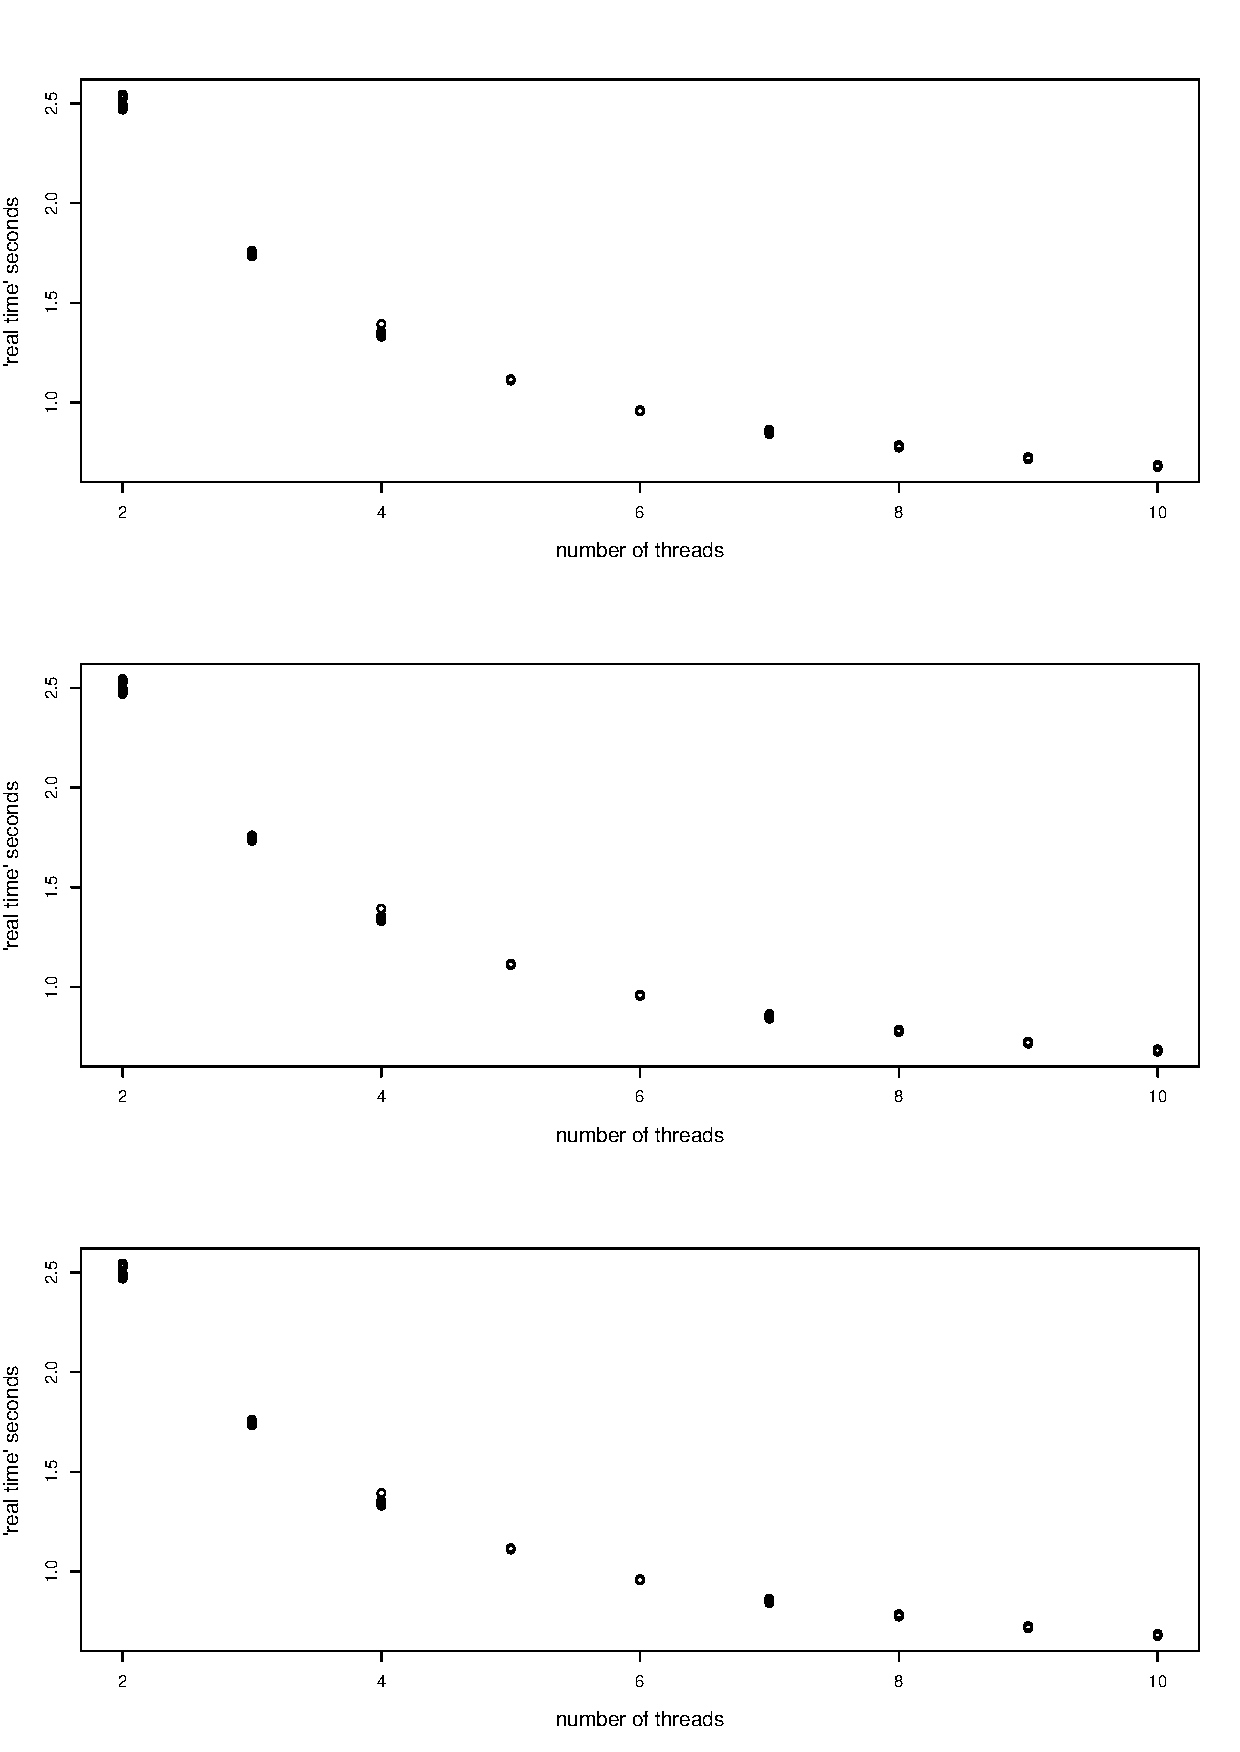
\includegraphics[width=\textwidth]{perform.pdf}
\caption{\textit{This figure shows the execution time in relation to number of threads.}}
\label{fig:perform}
\end{figure}




\addcontentsline{toc}{section}{\refname}
\bibliography{references}

\end{document}
